\documentclass[a4paper,11pt]{article}
\newlength{\outerbordwidth}
\pagestyle{empty}
\raggedbottom
\raggedright
\usepackage[svgnames]{xcolor}
\usepackage{framed}
\usepackage{times}
\usepackage{tocloft}
\usepackage{graphicx}
\usepackage{multirow}
\usepackage[utf8]{inputenc}
\usepackage{tabularx}
\usepackage{tabu}
\title{Resume}

\definecolor{shadecolor}{gray}{0.2}  % Outer background color of title bars (0 = black, 1 = white)
\definecolor{shadecolorB}{gray}{1}  % Inner background color of title bars

%Margin setup

\setlength{\evensidemargin}{-0.25in}
\setlength{\headheight}{0in}
\setlength{\headsep}{0in}
\setlength{\oddsidemargin}{-0.25in}
\setlength{\paperheight}{11in}
\setlength{\paperwidth}{8.5in}
\setlength{\tabcolsep}{0in}
\setlength{\textheight}{9.5in}
\setlength{\textwidth}{7in}
\setlength{\topmargin}{-0.3in}
\setlength{\topskip}{0in}
\setlength{\voffset}{0.1in}

\newcommand{\resitem}[1]{\item #1 \vspace{-2pt}}
\newcommand{\resheading}[1]{\vspace{8pt}
	\parbox{\textwidth}{\setlength{\FrameSep}{\outerbordwidth}
		\begin{shaded}
			\setlength{\fboxsep}{0pt}\framebox[\textwidth][l]{\setlength{\fboxsep}{4pt}\fcolorbox{shadecolorB}{shadecolorB}{\textbf{\sffamily{\mbox{~}\makebox[6.762in][l]{\large #1} \vphantom{p\^{E}}}}}}
		\end{shaded}
	}\vspace{-5pt}
}
\newcommand{\ressubheading}[4]{
	
	\begin{tabular*}{6.5in}{l@{\cftdotfill{\cftsecdotsep}\extracolsep{\fill}}r}
		\textbf{#1} & #2 \\
		\textit{#3} & \textit{#4} \\
	\end{tabular*}\vspace{-6pt}}

\begin{document}
	 %Profile photo 
	\begin{tabular*}{7in}{l@{\extracolsep{\fill}}r}
		& \multirow{1}{*}{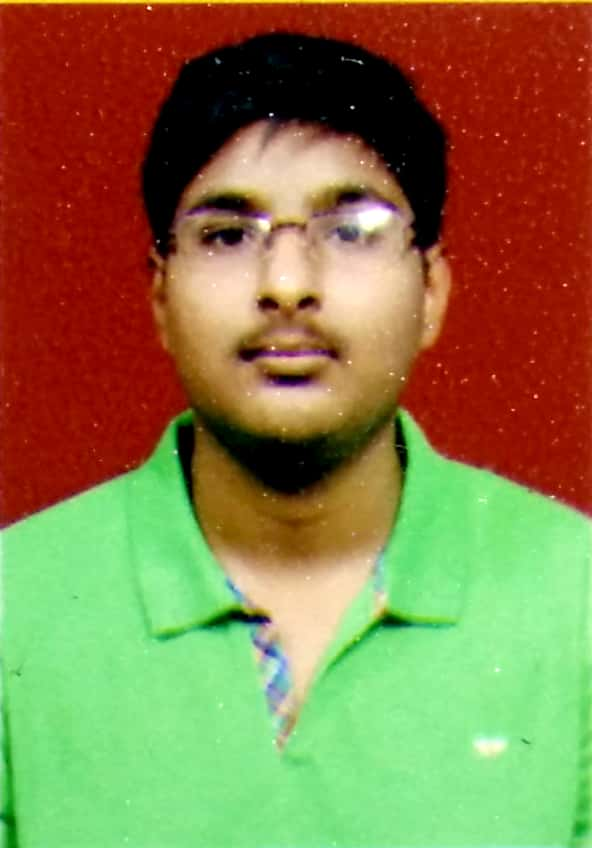
\includegraphics[scale=0.11]{Profile}}\\
		\\
		%Details
		\textbf{\Large Priyank Shah  } & \\
		6, Mahalaxmi Mansion, C.P.Tank, 2nd floor, room no 36, Mumbai-4. \\
		priyank.shah998@gmail.com \\
		+91-8639045967\\
    \end{tabular*}
\\
\resheading{Objective}

\begin{itemize}
	\item
	To work in a challenging environment that demands constant development of fresh skills and maximum utilization of the existing skills, as well as achieve the goals of the organization.
\end{itemize}
	
	\resheading{Education}
	
	\begin{tabu} to 1\textwidth { | X[c] | X[c] | X[c] | X[c] | X[c] |}
		\hline
		\textbf{Degree} & \textbf{College /School} & \textbf{University} & \textbf{Passing Year} & \textbf{Pass Percentage}\\ 
		\hline
		BE. Info Tech. & Fr.Conceicao Rodrigues College Of Engineering, Bandra & Mumbai University & 2019 & 9.24 (Till Sem V) \\
		\hline
		HSC & K C College, Churchgate & Maharashtra Board & 2015 & 84.62\%\\
		\hline
		SSC & St.Xavier's Boys' Academy, Marine Lines & Maharashtra Board & 2013 & 89.82\%\\
		\hline
	\end{tabu}

\resheading{Project}

\begin{itemize}
	\item{\textbf{Automatic Traffic Surveillance System}}
	\begin{itemize}
		\resitem{Project aims to identify different types of traffic offenders like signal and helmet offenders, over speeders, etc.}
		\resitem{Worked on object detection module which mainly focuses on detection of vehicles and helmets.}
		\resitem{Implemented using Tflearn, OpenCV and Python}
	\end{itemize}
\end{itemize}
	
\end{document}